\documentclass[10pt,a4paper,onecolumn]{article}
% \usepackage[utf8]{inputenc}
\usepackage{marginnote}
\usepackage{graphicx}
\usepackage{xcolor}
\usepackage{authblk,etoolbox}
\usepackage{titlesec}
\usepackage{calc}
\usepackage{hyperref}
\hypersetup{breaklinks=true,
            bookmarks=true,
            pdfauthor=
{
      Mario Senden,
      Jannis Schuecker,,
      Jan Hahne,,
      Markus Diesmann,,
      Rainer Goebel,,
  },
            pdftitle=
{
[Re] A neural model of the saccade generator in the reticular formation
},
            colorlinks=true,
            citecolor=blue,
            urlcolor=blue,
            linkcolor=blue,
            pdfborder={0 0 0}}
\urlstyle{same}
\usepackage{tcolorbox}
\usepackage{ragged2e}
\usepackage{fontspec}
\usepackage{fontawesome}
\usepackage{caption}
\usepackage{listings}
\lstnewenvironment{code}{\lstset{language=Haskell,basicstyle=\small\ttfamily}}{}



%\usepackage{fancyvrb}
%\VerbatimFootnotes
%\usepackage{graphicx}
%\usepackage{mdframed}
%\newmdenv[backgroundcolor=lightgray]{Shaded}


\usepackage{longtable,booktabs}

\usepackage[
  backend=biber,
%  style=alphabetic,
%  citestyle=numeric
]{biblatex}
\bibliography{senden-schuecker-hahne-diesmann-goebel-2017.bib}



% --- Macros ------------------------------------------------------------------
\renewcommand*{\bibfont}{\small \sffamily}

\definecolor{red}{HTML}{CF232B}
\newcommand{\ReScience}{Re{\bfseries \textcolor{red}{Science}}}

\newtcolorbox{rebox}
   {colback=blue!5!white, colframe=blue!40!white,
     boxrule=0.5pt, arc=2pt, fonttitle=\sffamily\scshape\bfseries,
     left=6pt, right=20pt, top=6pt, bottom=6pt}

\newtcolorbox{repobox}
   {colback=red, colframe=red!75!black,
     boxrule=0.5pt, arc=2pt, left=6pt, right=6pt, top=3pt, bottom=3pt}

% fix for pandoc 1.14     
\newcommand{\tightlist}{%
  \setlength{\itemsep}{1pt}\setlength{\parskip}{0pt}\setlength{\parsep}{0pt}}

% --- Style -------------------------------------------------------------------
\renewcommand*{\bibfont}{\small \sffamily}
\renewcommand{\captionfont}{\small\sffamily}
\renewcommand{\captionlabelfont}{\bfseries}

\makeatletter
\renewcommand\@biblabel[1]{{\bf #1.}}
\makeatother

% --- Page layout -------------------------------------------------------------
\usepackage[top=3.5cm, bottom=3cm, right=1.5cm, left=1.5cm,
            headheight=2.2cm, reversemp, includemp, marginparwidth=4.5cm]{geometry}

% --- Section/SubSection/SubSubSection ----------------------------------------
\titleformat{\section}
  {\normalfont\sffamily\Large\bfseries}
  {}{0pt}{}
\titleformat{\subsection}
  {\normalfont\sffamily\large\bfseries}
  {}{0pt}{}
\titleformat{\subsubsection}
  {\normalfont\sffamily\bfseries}
  {}{0pt}{}
\titleformat*{\paragraph}
  {\sffamily\normalsize}


% --- Header / Footer ---------------------------------------------------------
\usepackage{fancyhdr}
\pagestyle{fancy}
%\renewcommand{\headrulewidth}{0.50pt}
\renewcommand{\headrulewidth}{0pt}
\fancyhead[L]{\hspace{-1cm}\includegraphics[width=4.0cm]{rescience-logo.pdf}}
\fancyhead[C]{}
\fancyhead[R]{} 
\renewcommand{\footrulewidth}{0.25pt}

\fancyfoot[L]{\hypersetup{urlcolor=red}
              \sffamily \ReScience~$\vert$
              \href{http://rescience.github.io}{rescience.github.io}
              \hypersetup{urlcolor=blue}}
\fancyfoot[C]{\sffamily \thepage}
\fancyfoot[R]{\sffamily Month 2017 $\vert$
                        Volume \textbf{1} $\vert$
                        Issue \textbf{1}}
\pagestyle{fancy}
\makeatletter
\let\ps@plain\ps@fancy
\fancyheadoffset[L]{4.5cm}
\fancyfootoffset[L]{4.5cm}

% --- Title / Authors ---------------------------------------------------------
% patch \maketitle so that it doesn't center
\patchcmd{\@maketitle}{center}{flushleft}{}{}
\patchcmd{\@maketitle}{center}{flushleft}{}{}
% patch \maketitle so that the font size for the title is normal
\patchcmd{\@maketitle}{\LARGE}{\LARGE\sffamily}{}{}
% patch the patch by authblk so that the author block is flush left
\def\maketitle{{%
  \renewenvironment{tabular}[2][]
    {\begin{flushleft}}
    {\end{flushleft}}
  \AB@maketitle}}
\makeatletter
\renewcommand\AB@affilsepx{ \protect\Affilfont}
%\renewcommand\AB@affilnote[1]{{\bfseries #1}\hspace{2pt}}
\renewcommand\AB@affilnote[1]{{\bfseries #1}\hspace{3pt}}
\makeatother
\renewcommand\Authfont{\sffamily\bfseries}
\renewcommand\Affilfont{\sffamily\small\mdseries}
\setlength{\affilsep}{1em}

\LetLtxMacro{\OldIncludegraphics}{\includegraphics}
\renewcommand{\includegraphics}[2][]{\OldIncludegraphics[width=12cm, #1]{#2}}


% --- Document ----------------------------------------------------------------
\title{[Re] A neural model of the saccade generator in the reticular formation}

    \usepackage{authblk}
                        \author[1, 2]{Mario Senden}
                    \author[3]{Jannis Schuecker,}
                    \author[4]{Jan Hahne,}
                    \author[3, 5, 6]{Markus Diesmann,}
                    \author[1, 2, 7]{Rainer Goebel,}
                            \affil[1]{Department of Cognitive Neuroscience, Faculty of Psychology and
Neuroscience, Maastricht University, 6201BC Maastricht, The Netherlands}
                    \affil[2]{Maastricht Brain Imaging Centre, Faculty of Psychology and Neuroscience,
Maastricht University, P.O. Box 616, 6200 MD Maastricht, The Netherlands}
                    \affil[3]{Institute of Neuroscience and Medicine (INM-6) and Institute for
Advanced Simulation (IAS-6) and JARA BRAIN Institute I, Jülich Research
Centre, 52428 Jülich, Germany}
                    \affil[4]{School of Mathematics and Natural Sciences, Bergische Universit"at
Wuppertal, Wuppertal, Germany}
                    \affil[5]{Department of Psychiatry, Psychotherapy and Psychosomatics, Medical
Faculty, RWTH Aachen University, 52062 Aachen, Germany}
                    \affil[6]{Department of Physics, Faculty 1, RWTH Aachen University, 52062 Aachen,
Germany}
                    \affil[7]{Department of Neuroimaging and Neuromodeling, Netherlands Institute for
Neuroscience, an Institute of the Royal Netherlands Academy of Arts and
Sciences (KNAW), 1105BA Amsterdam, The Netherlands}
            
\date{\vspace{-5mm}
      \sffamily \small \href{mailto:mario.senden@maastrichtuniversity.nl}{mario.senden@maastrichtuniversity.nl}}


\setlength\LTleft{0pt}
\setlength\LTright{0pt}


\begin{document}
\maketitle

\marginpar{
  %\hrule
  \sffamily\small
  %\vspace{2mm}
  {\bfseries Editor}\\
  Name Surname\\

  {\bfseries Reviewers}\\
        Name Surname\\
        Name Surname\\
  
  {\bfseries Received}  Month, Day, 2017\\
  {\bfseries Accepted}  Month, Day, 2017\\
  {\bfseries Published} Month, Day, 2017\\

  {\bfseries Licence}   \href{http://creativecommons.org/licenses/by/4.0/}{CC-BY}

  \begin{flushleft}
  {\bfseries Competing Interests:}\\
  The authors have declared that no competing interests exist.
  \end{flushleft}

  \hrule
  \vspace{3mm}

  \hypersetup{urlcolor=white}
  
    \vspace{-1mm}
  \begin{repobox}
    \bfseries\normalsize
      \href{http://github.com/rescience/rescience-submission/article}{\faGithubAlt~Article repository}
  \end{repobox}
      \vspace{-1mm}
  \begin{repobox}
    \bfseries\normalsize
      \href{http://github.com/rescience/rescience-submission/code}{\faGithubAlt~Code repository}
  \end{repobox}
        \hypersetup{urlcolor=blue}
}

\begin{rebox}
\sffamily {\bfseries A reference implementation of}
\small
\begin{flushleft}
\begin{itemize}
    \item[→] \emph{A neural model of the saccade generator in the reticular
formation}, G. Gancarz, S. Grossberg, Neural Networks, 1159-1174, 1998
  \end{itemize}\par
\end{flushleft}
\end{rebox}


\section{Introduction}\label{introduction}

We provide an implementation of the saccade generator (SG); a rate
neuron model of the neural circuitry in the reticular formation proposed
by Gancarz \& Grossberg \autocite{Gancarz1998}. The same group has
recently sucessfully embedded the SG into a larger model of the eye
movement network \autocite{Grossberg2012} showcasing its compatible
nature. This compatibility of the SG model might prove useful in the
future for studying the interplay of neural (sub)systems of visuo-motor
integration. It is thus of interest to implement the model in publicly
available, widely used, and actively developed neural simulation
frameworks such as NEST \autocite{Gewaltig2007}. We show that the model
translates well to the NEST framework as our implementation faithfully
reproduces most simulation results reported in the original publication.
Our code uses the Python interface \autocite{Eppler2008} for legibility
with both model and analysis scripts being implemented using Python
2.7.12.

\section{Methods}\label{methods}

The SG model described by Gancarz \& Grossberg \autocite{Gancarz1998}
consists of a horizontal and a vertical component each with two
long-lead burst neurons (LLBNs), excitatory burst neurons (EBNs),
inhibitory burst neurons (IBNs), and tonic neurons (TNs). Within each
component, the two directions (left-right, down-up) interact
antagonistically. Additionally, both components share a single omnipause
neuron (OPN) which tonically inhibits each EBN as long as no saccade is
being initiated. In implementing this model, we largely followed the
descriptions provided in the original publication with a number of
well-motivated exceptions. First, in the original description, neuron
activations are bounded from below at zero implying their rectification
at every step during numerical integration. Instead, we opted for
passing all inputs received by a neuron through a rectified linear gain
function prior to their summation. Second, we replaced the gain function
given by equation A11 in the original publication
\begin{equation} g(x) = {\frac{x^4}{0.1^4+x^4}} \label{eq:eqn_1}\end{equation}
by
\begin{equation} g(x) = {\frac{1}{1+e^{-40(x-0.1)}}} \label{eq:eqn_2}\end{equation}
to prevent positive responses to negative net input. Otherwise equation
\ref{eq:eqn_2} closely approximates the shape of equation \ref{eq:eqn_1}
for \(\mathrm{x>0}\). Third, according to equation A12 in the original
publication, horizontal eye position is given by
\(\mathrm{\theta=260({TN}_{r}-0.5)}\). However, omitting rectification
in our implementation, allowed us to set activation of TNs to 0 rather
than 0.5 when the eye is at the center of its range. Finally, the
original implementation uses the fourth order Runge--Kutta method for
numerical integration. Instead, we used the Exponential Euler method
which is standardly implemented in NEST 1.1.x.x for numerical
integration of rate neurons \autocite{Hahne2016}.

In addition to these changes, the original model description has two
features which cannot be straightforwardly translated to NEST. First, a
nonlinear gain function is applied to a subset of inputs to EBNs and the
OPN while a linear gain function is applied to their remaining inputs.
Since NEST only applies a single gain function per neuron to each of its
inputs, we opted for using a (rectified) linear gain function for EBNs
and the OPN. In addition, we passed those inputs requiring an additional
nonlinear gain function through an auxiliary unit instantaneously
applying the desired nonlinearity before passing the result on to EBNs
and the OPN. Second, constant input to a neuron was not hard-coded but
rather provided by an appropriately weighted bias node.

In all simulations we used a time step of \(0.001\,\mathrm{ms}\) and a
time constant of \(50\,\mathrm{ms}\). It should be noted that rates of
all neurons were initialized to zero and were thus not at resting
equilibrium. In order to address this, the model was allowed to evolve
for \(50\,\mathrm{ms}\), to reach equilibrium before applying any input.
Furthermore, we always simulated the full model; i.e.~both its
horizontal and vertical components even if input was applied only to one
of the two.

\section{Results}\label{results}

All results from the original publication have been implemented. Our
results accord very well with those reported by Gancarz \& Grossberg
\autocite{Gancarz1998}. Nevertheless, some inconsistencies exist and
will be discussed.

The first simulation reported in Gancarz \& Grossberg
\autocite{Gancarz1998} showcases the evolution of activity for each
neuron type in the horizontal SG to a constant input (\(\mathrm{I=1}\))
applied to the left LLBN for \(265\,\mathrm{ms}\). The original
publication does not report exact activation values observed for each
neuron rendering a quantitative analysis of the accuracy of our
replication impossible. However, qualitatively activation profiles shown
in figure 3 in the original publication and those shown in figure
\ref{fig:fig_1} show good correspondence. A noticeable difference is
that rectification in the original publication would prohibit neuron
activations from exhibiting negative values. In our implementation
negative values are possible and clearly exhibited by EBNs. Since we
apply a rectified linear gain function, however, these negative values
have a negligible effect on the behavior of the system as a whole.

\begin{figure}
\centering
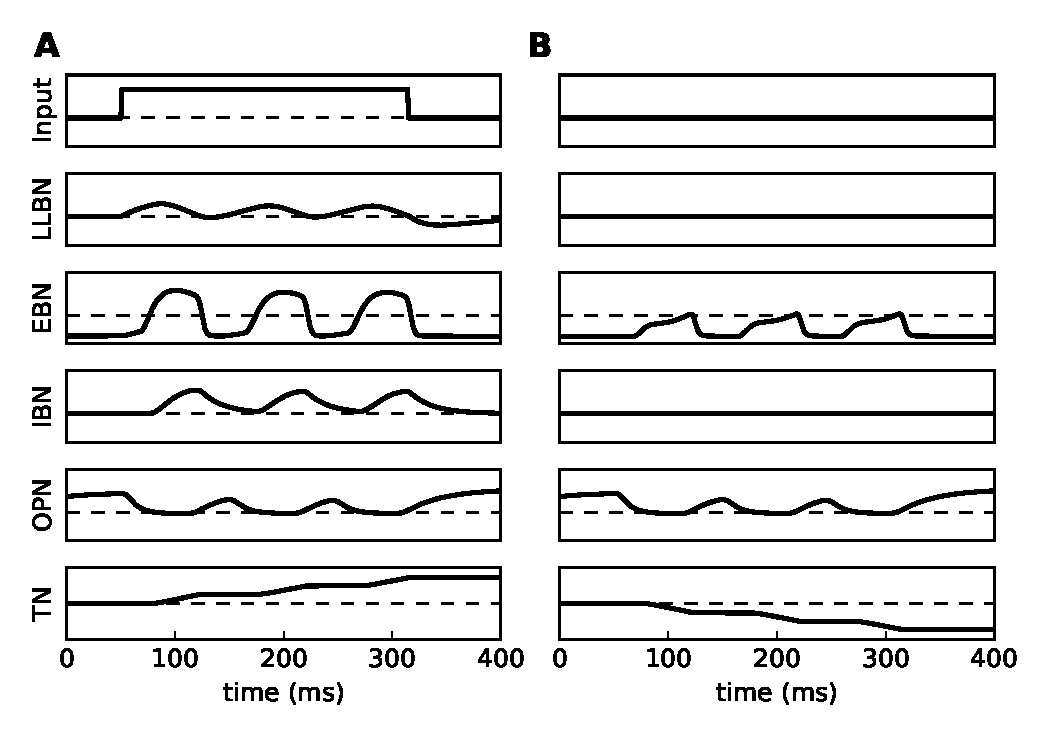
\includegraphics[width=0.75000\textwidth,height=0.45000\textwidth]{../code/fig1.eps}
\caption{\textbf{Activity profiles in the left (A) and right (B) SG.}
All activities are in response to constant input applied to the left
LLBN. The dashed horizontal line marks zero. Excitatory burst neurons
(EBNs) exhibit negative baseline activity.\label{fig:fig_1}}
\end{figure}

The second simulation shows the relation between input strength and
burst amplitude for LLBNs and EBNs. Inputs to the left SG were equal to
\(\mathrm{I=1}\) (figure \ref{fig:fig_2}, blue), \(\mathrm{I=1.75}\)
(figure \ref{fig:fig_2}, green), and \(\mathrm{I=2.5}\) (figure
\ref{fig:fig_2}, red); each applied to the left LLBN for
\(85\,\mathrm{ms}\). Qualitatively, our results accord well with those
shown in figure 5 of the original publication. As before, our results
differ only with respect to the possibility of negative activity values.

\begin{figure}
\centering
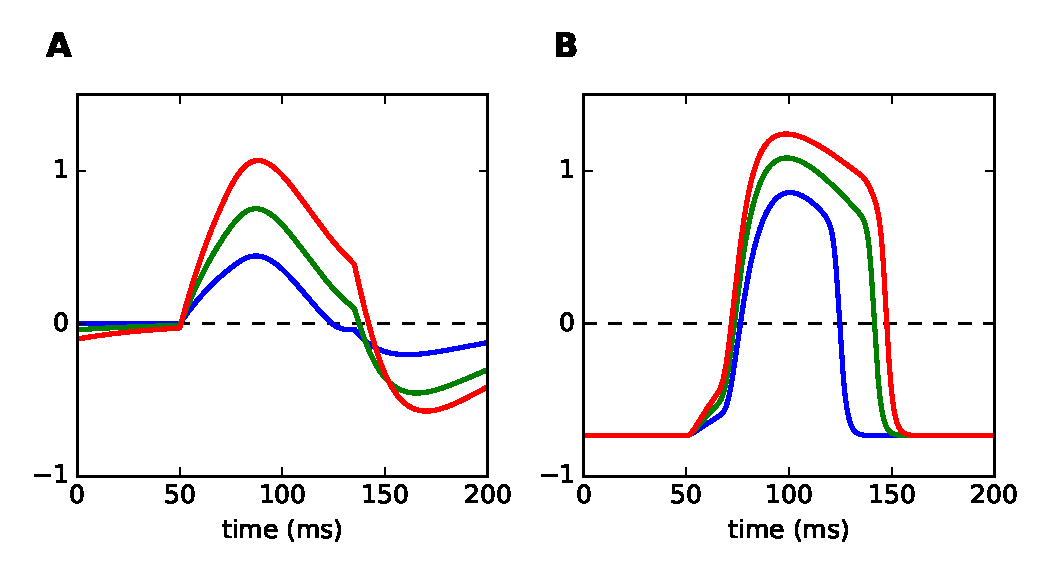
\includegraphics[width=0.75000\textwidth,height=0.36000\textwidth]{../code/fig2.eps}
\caption{\textbf{Activity profiles in LLBN (A) and EBN (B).} Increased
input strength results in larger LLBN and EBN burst size with inputs
equal to 1 (blue), 1.75 (green), and 2.5 (red).\label{fig:fig_2}}
\end{figure}

The third simulation produces saccades in response to different input
strengths to the horizontal and vertical SG. Specifically, inputs to the
right and upward LLBNs were (\(\mathrm{{I}_{r}=0.67}\),
\(\mathrm{{I}_{u}=0.08}\); figure \ref{fig:fig_3}, blue),
(\(\mathrm{{I}_{r}=0.7}\), \(\mathrm{{I}_{u}=0.22}\); figure
\ref{fig:fig_3}, green), (\(\mathrm{{I}_{r}=0.74}\),
\(\mathrm{{I}_{u}=0.4}\); figure \ref{fig:fig_3}, red),
(\(\mathrm{{I}_{r}=0.75}\), \(\mathrm{{I}_{u}=0.6}\); figure
\ref{fig:fig_3}, turqoiuse), and (\(\mathrm{{I}_{r}=0.7}\),
\(\mathrm{{I}_{u}=0.9}\); figure \ref{fig:fig_3}, purple). Inputs to the
horizontal and vertical SG were applied for \(75\,\mathrm{ms}\). Our
results are again in good agreement with those shown in figure 6 of the
original publication.

\begin{figure}
\centering
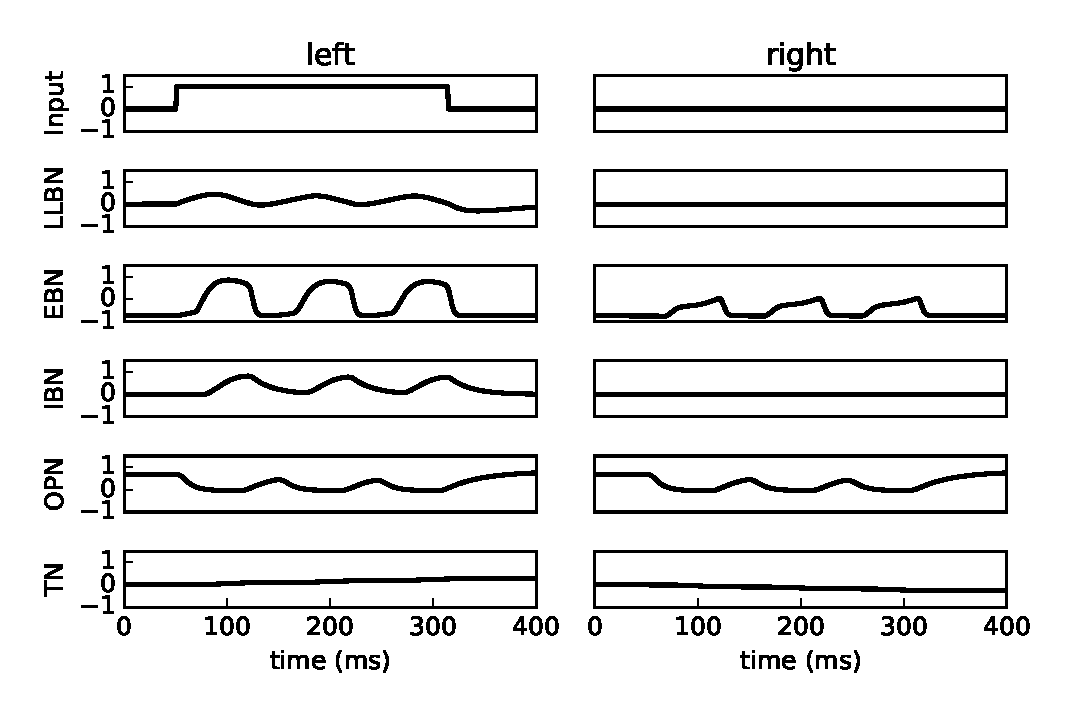
\includegraphics[width=0.48750\textwidth,height=0.48750\textwidth]{../code/fig3.eps}
\caption{\textbf{Oblique saccades.} Saccades are fairly straight with a
slight tendency to curve.\label{fig:fig_3}}
\end{figure}

The fourth simulation generates a staircase of three saccades in
response to continuous input. Here, inputs to the right and upward LLBNs
were equal to \(\mathrm{{I}_{r}=0.2}\) and \(\mathrm{{I}_{u}=0.33}\) for
\(300\,\mathrm{ms}\). In the original implementation, the input was
presented for \(250\,\mathrm{ms}\). However, this lead to the production
of two rather than three saccades in our implementation motivating the
choice of a slightly longer stimulation period. Another difference is
that our implementation produces slightly larger saccades. Specifically,
after the first saccade horizontal and vertical eye positions are
respectively at 4\textdegree~and 6\textdegree~in our simulation while
they are at \(\sim3\)\textdegree~and \(\sim5\)\textdegree~in the
original publication. Similarly, after the second saccade horizontal and
vertical eye positions are respectively at 7\textdegree~and
12\textdegree~in our simulation while they are at
\(\sim6\)\textdegree~and \(\sim9\)\textdegree~in the original
publication.

\begin{figure}
\centering
\includegraphics[width=0.33000\textwidth,height=0.45000\textwidth]{../code/fig4.eps}
\caption{\textbf{Saccadic staircase.} Three saccades in a staircase
continue in the same direction as the initial saccade. Eye position was
sampled every \(2\,\mathrm{ms}\).\label{fig:fig_4}}
\end{figure}

In the fifth simulation the average activity of the left EBN is obtained
for a series of saccades with different directions. Note that for
reasons of comparability with the original publication, only positive
activation values were averaged. Figure \ref{fig:fig_5} shows a polar
plot of average activity corresponding to each saccade reflecting the
neuron's tuning curve. The inputs to the SG producing the desired
saccades can be found in table \ref{tbl:table_1}. Each of these inputs
was applied for \(50\,\mathrm{ms}\). The tuning curve we observe for the
left EBN exhibits a cardioid-like shape as was the case in the original
publication.

\begin{figure}
\centering
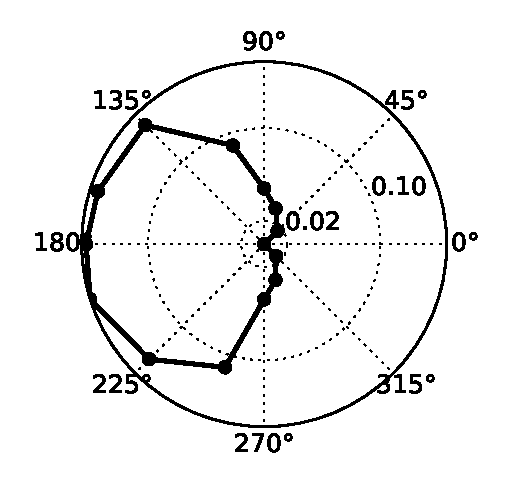
\includegraphics[width=0.37500\textwidth,height=0.37500\textwidth]{../code/fig5.eps}
\caption{\textbf{EBN tuning curve.} Tuning curve of the left EBN
exhibiting a cardioid-like shape.\label{fig:fig_5}}
\end{figure}

\begin{longtable}[]{@{}lllllllllllllll@{}}
\caption{Direction specific inputs to SG to produce EBN tuning curve.
\label{tbl:table_1}}\tabularnewline
\toprule
& 0 & 45 & 72 & 90 & 108 & 135 & 162 & 180 & 198 & 225 & 252 & 270 & 288
& 315\tabularnewline
\midrule
\endfirsthead
\toprule
& 0 & 45 & 72 & 90 & 108 & 135 & 162 & 180 & 198 & 225 & 252 & 270 & 288
& 315\tabularnewline
\midrule
\endhead
\(\mathrm{{I}_{l}}\) & .00 & .00 & .00 & .00 & .20 & .45 & .63 & .70 &
.63 & .45 & .20 & .00 & .00 & .00\tabularnewline
\(\mathrm{{I}_{r}}\) & .70 & .45 & .20 & .00 & .00 & .00 & .00 & .00 &
.00 & .00 & .00 & .00 & .20 & .45\tabularnewline
\(\mathrm{{I}_{d}}\) & .00 & .00 & .00 & .00 & .00 & .00 & .00 & .00 &
.20 & .45 & .63 & .70 & .63 & .45\tabularnewline
\(\mathrm{{I}_{u}}\) & .00 & .45 & .63 & .70 & .63 & .45 & .20 & .00 &
.00 & .00 & .00 & .00 & .00 & .00\tabularnewline
\bottomrule
\end{longtable}

The sixth simulation reported in the original publication is designed to
replicate results of Stanford \textit{et al.} \autocite{Stanford1996}.
These authors stimulated the superior colliculus (SC) at various
frequencies and measured the resulting saccade amplitude, duration, and
velocity; showing that ampltidude saturates before velocity. Our
implementation of the SG model was capable of replicating these results.
However, reproducing simulation results reported by Gancarz \& Grossberg
\autocite{Gancarz1998} with our implementation was complicated by the
fact that the stimulation protocol given by the authors lead to the
production of two rather than a single saccade. Furthermore, the authors
did not report their criteria for identifying saccade on- and offsets.
Stanford \textit{et al.} \autocite{Stanford1996} used velocity criteria
to determine onset (\(v\textgreater30\,\mathrm{deg/s}\)) and offset
(\(v\textless30\,\mathrm{deg/s}\)) of a saccade. While this provided us
with explicit criteria, velocity did not always drop below
\(30\,\mathrm{deg/s}\) after the first saccade before rising again with
the second. To determine the offset of a saccade in those cases, we
found the local minimum between the end of the first and the beginning
of the second saccade. With these criteria in place, we stimulated the
SC at a frequency varying between 1 and 2.4 at increments of 0.2. The
connection weight from SC to LLBN was set equal to two and stimulation
duration was \(125\,\mathrm{ms}\). Results of our simulation are shown
in figure \ref{fig:fig_6} and accord well with those reported in the
original publication (their figure 9). Interestingly, saccade amplitude
in response to a stimulation frequency of 1.2 in the original
implementation is larger than expected given both our simulation and
empirical results. It is possible that the offset criterion employed by
Gancarz \& Grossberg \autocite{Gancarz1998} failed to differentiate
between two saccades following each other in very short succession
leading to an overestimation of saccade duration.

\begin{figure}
\centering
\includegraphics[width=0.75000\textwidth,height=0.37500\textwidth]{../code/fig6.eps}
\caption{\textbf{Effect of stimulation frequency on saccade (A)
amplitude, (B) duration, and (C) velocity.} Saccade amplitude (A)
saturates before saccade velocity (C).\label{fig:fig_6}}
\end{figure}

\pagebreak

The seventh simulation shows that saccade velocity and duration can be
traded while keeping amplitude constant. To produce a high-velocity
saccade, the SC was stimulated with a frequency \(\mathrm{F=3}\) for
\(62\,\mathrm{ms}\). Similarly, to produce a low-velocity saccade, the
SC was stimulated with a frequency of \(\mathrm{F=1.3}\) for
\(112\,\mathrm{ms}\). The stimulation duration was in both cases shorter
than those reported by Gancarz \& Grossberg \autocite{Gancarz1998}
(\(82\,\mathrm{ms}\) and \(117\,\mathrm{ms}\)) to reproduce the behavior
of the SC shown in their figure 10 more faithfully. Figure
\ref{fig:fig_7} shows the results of our simulation. In accordance with
the original simulation, saccade amplitude reflected by TN activity was
identical after high- and low-frequency saccades. However, our
implementation produced a second, small, saccade not observed for the
original implementation.

\begin{figure}
\centering
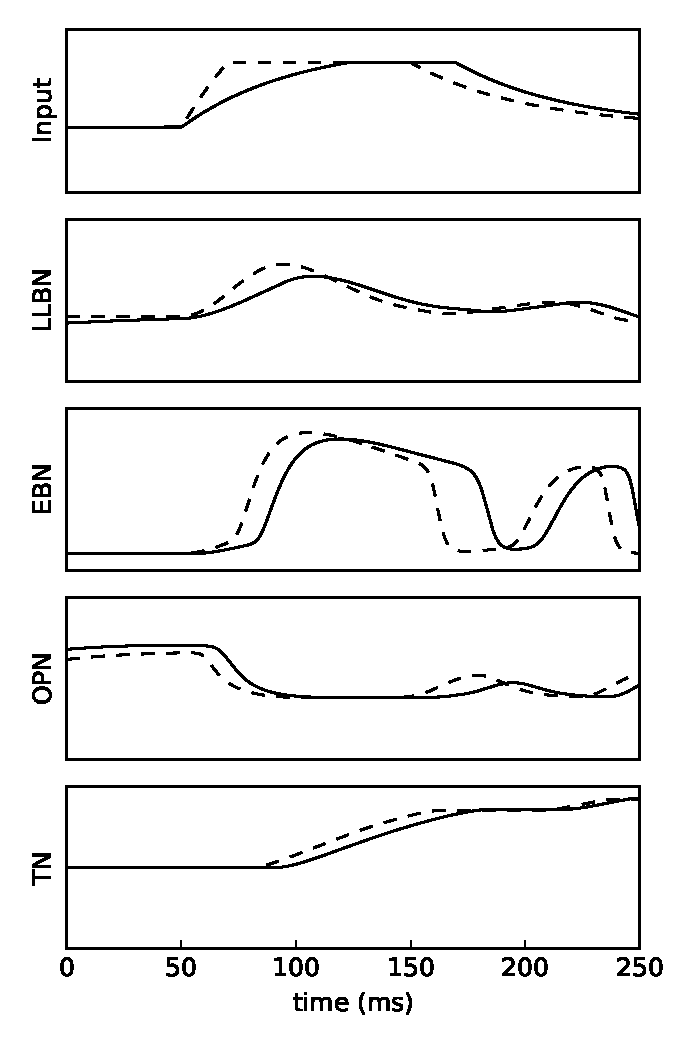
\includegraphics[width=0.49500\textwidth,height=0.75000\textwidth]{../code/fig7.eps}
\caption{\textbf{Trading saccade velocity for duration.} Duration and
velocity of a saccade can be traded while keeping amplitude constant
given an appropriate shape of the input signal.\label{fig:fig_7}}
\end{figure}

The eighth simulation reported by Gancarz \& Grossberg
\autocite{Gancarz1998} shows how strong (\(\mathrm{I=3}\)) sustained
(\(300\,\mathrm{ms}\)) input to the SG produces a single large saccade
followed by a series of small saccades resembling smooth eye movements.
Our results, shown in figure \ref{fig:fig_8}, reproduce these findings
as they strongly resemble those shown in figure 11 of the original
publication.

\begin{figure}
\centering
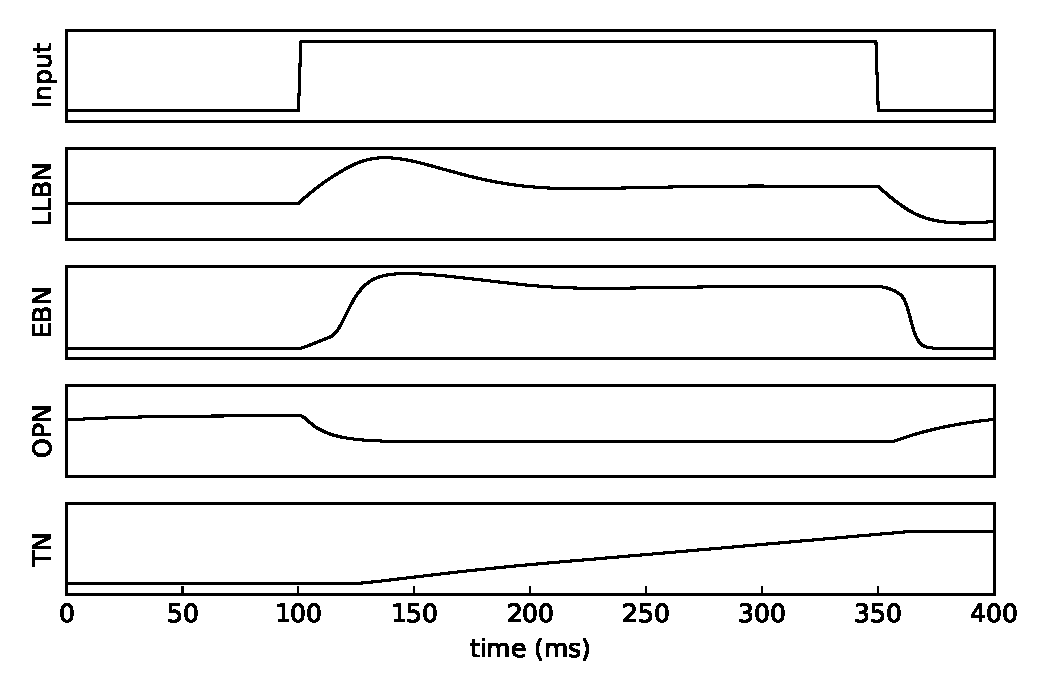
\includegraphics[width=0.75000\textwidth,height=0.49500\textwidth]{../code/fig8.eps}
\caption{\textbf{Smooth staircase eye movements.} Activity profiles of
SG neurons accompanying a single saccade followed by smooth eye movement
as a result of strong sustained input.\label{fig:fig_8}}
\end{figure}

The final simulation showcases the evolution of activity exhibited by SG
neurons when the OPN was electrically stimulated (\(\mathrm{J=1.8}\))
for \(5\,\mathrm{ms}\) while a constant input (\(\mathrm{I=0.7}\)) was
applied to the LLBN for \(100\,\mathrm{ms}\). External stimulation
temporarily restored activation in the OPN and hence also inhibition of
the EBN, leading to an interruption of the saccade. As is shown in
figure \ref{fig:fig_9}, the saccade remained accurate despite this
disruption. This is in agreement with results shown in figure 12 of the
original publication.

\begin{figure}
\centering
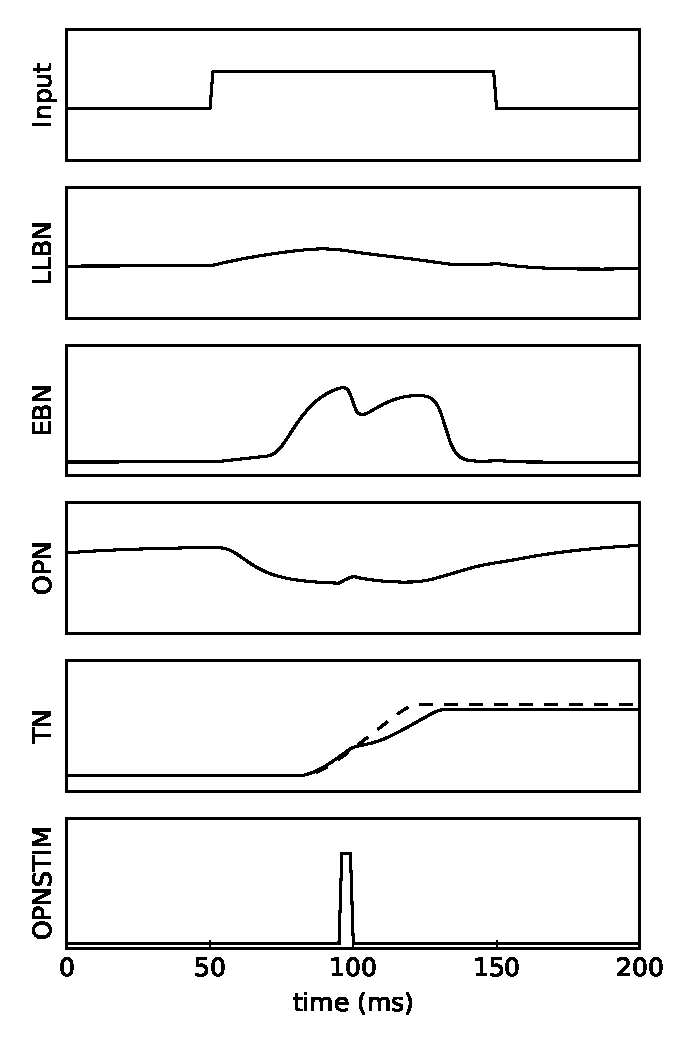
\includegraphics[width=0.49500\textwidth,height=0.75000\textwidth]{../code/fig9.eps}
\caption{\textbf{Interrupted saccade resulting from OPN stimulation.}
OPN stimulation interrupts the saccade, which remains accurate
nonetheless. The dashed line shows TN activity for an uninterrupted
saccade.\label{fig:fig_9}}
\end{figure}

\section{Conclusion}\label{conclusion}

The reproduced results generally show good qualitative correspondence
with those reported by Gancarz and Grossberg \autocite{Gancarz1998} and
accorded well quantitatively whenever such information was available.
One notable difference is that EBNs in our implementation exhibited
negative activity levels at baseline since we did not artificially bound
them from below at zero. While this constitutes a significant change to
the model, any effects this might have had were offset by passing inputs
to each neuron through a rectified linear gain function rather than
summing them linearly. furthermore, our implementation produced saccades
of slighly larger amplitude than the original implementation. This was
likely due to the different choice of gain function applied to the
inputs of the OPN. Specifically, our gain function has a steeper slope
which caused the OPN to shut-off faster in response to LLBN activty
which, in turn, lead to prolonged release from inhibition of EBNs. These
effects were minute but sufficient to cause differences in saccade
amplitude of \(\sim1\)\textdegree.

In conclusion, our reproduction confirms the results of the original
publication and shows that an implementation in the NEST framework is
feasible. This allows for the straightforward integration of the saccade
generator into models of the visuomotor system forming the interface
between sensory processing and motor control.

\section{Acknowledgments}\label{acknowledgments}

All network simulations carried out with NEST
(http://www.nest-simulator.org).

{\sffamily \small
  \printbibliography[title=References]
}
\end{document}
